\documentclass[a4paper, 12pt]{article}

\usepackage[T2A]{fontenc}
\usepackage[utf8]{inputenc}
% \usepackage[portuges]{babel}
\usepackage{amsmath,amssymb}
\usepackage{graphicx}
\graphicspath{{/images}}
\usepackage{subfig}
\setlength {\marginparwidth }{2cm}
\usepackage[colorinlistoftodos]{todonotes}
\usepackage{float}%"Плавающие" картинки
\usepackage{wrapfig}%Обтекание фигур (таблиц, картинок и прочего)

\usepackage{indentfirst}
\usepackage{listings}
\usepackage{caption}
\usepackage{pifont}
\usepackage{relsize}
\usepackage{etoolbox}
\usepackage{color}
\usepackage{sectsty}
\allsectionsfont{\centering}

\definecolor{mygreen}{rgb}{0,0.6,0}
\definecolor{mygray}{rgb}{0.5,0.5,0.5}
\definecolor{mymauve}{rgb}{0.58,0,0.82}

\lstset{ %
  backgroundcolor=\color{white},   % choose the background color; you must add \usepackage{color} or \usepackage{xcolor}
  basicstyle=\footnotesize,        % the size of the fonts that are used for the code
  breakatwhitespace=false,         % sets if automatic breaks should only happen at whitespace
  breaklines=true,                 % sets automatic line breaking
  captionpos=b,                    % sets the caption-position to bottom
  commentstyle=\color{mygreen},    % comment style
  deletekeywords={...},            % if you want to delete keywords from the given language
  escapeinside={\%*}{*)},          % if you want to add LaTeX within your code
  extendedchars=true,              % lets you use non-ASCII characters; for 8-bits encodings only, does not work with UTF-8
  frame=single,                    % adds a frame around the code
  keepspaces=true,                 % keeps spaces in text, useful for keeping indentation of code (possibly needs columns=flexible)
  keywordstyle=\color{blue},       % keyword style
  language=C++,                 % the language of the code
  otherkeywords={*,...},           % if you want to add more keywords to the set
  % numbers=left,                    % where to put the line-numbers; possible values are (none, left, right)
  % numbersep=5pt,                   % how far the line-numbers are from the code
  % numberstyle=\tiny\color{mygray}, % the style that is used for the line-numbers
  rulecolor=\color{black},         % if not set, the frame-color may be changed on line-breaks within not-black text (e.g. comments (green here))
  showspaces=false,                % show spaces everywhere adding particular underscores; it overrides 'showstringspaces'
  showstringspaces=false,          % underline spaces within strings only
  showtabs=false,                  % show tabs within strings adding particular underscores
  % stepnumber=2,                    % the step between two line-numbers. If it's 1, each line will be numbered
  stringstyle=\color{mymauve},     % string literal style
  tabsize=2,                       % sets default tabsize to 2 spaces
  title=\lstname                   % show the filename of files included with \lstinputlisting; also try caption instead of title
}
\patchcmd{\thebibliography}{\section*{\refname}}{}{}{}


\usepackage{lipsum}% http://ctan.org/pkg/lipsum
\usepackage{xcolor}% http://ctan.org/pkg/xcolor
\usepackage{xparse}% http://ctan.org/pkg/xparse
\NewDocumentCommand{\myrule}{O{1pt} O{2pt} O{black}}{%
  \par\nobreak % don't break a page here
  \kern\the\prevdepth % don't take into account the depth of the preceding line
  \kern#2 % space before the rule
  {\color{#3}\hrule height #1 width\hsize} % the rule
  \kern#2 % space after the rule
  \nointerlineskip % no additional space after the rule
}
\usepackage[section]{placeins}

\usepackage{booktabs}
\usepackage{colortbl}%
\newcommand{\myrowcolour}{\rowcolor[gray]{0.925}}

\usepackage[obeyspaces]{url}
\usepackage[colorlinks,citecolor=black,urlcolor=blue,bookmarks=false,hypertexnames=true]{hyperref}

\usepackage[a4paper, mag=1000, left=2cm, right=2cm, top=2cm, bottom=2cm, headsep=0.7cm, footskip=1cm]{geometry}
\usepackage[english,russian]{babel}
%*******************************************************************************%
%************************************START**************************************%
%*******************************************************************************%
\begin{document}
%************************************TITLE PAGE**************************************%
\begin{titlepage}
\begin{center}
\textsc{\normalsize ФГБОУ ВО «Национальный исследовательский Нижегородский
государственный университет им. Н.И. Лобачевского»
\vspace{5pt}
\break Институт Информационных технологий, математики и механики
\vspace{5pt}
\break Фундаментальная информатика и информационные технологии}\\



\vspace{150pt}
\textbf{\Large ОТЧЁТ ПО ЛАБОРАТОРНОЙ РАБОТЕ}\\
\vspace{15pt}

\textbf{\large «Построение выпуклой оболочки – проход Джарвиса.»}\\
\vspace{10pt}
\end{center}

\vspace{250pt}

\hfill
\begin{minipage}{.5\textwidth}
\textbf{Выполнил:\\[0.5mm]}
Студент 3 курса, группы 3821Б1ФИ3:
\break Иванов Никита Антонович\\[5mm]

\textbf{Проверил:\\[2mm]}
Нестеров Александр Юрьевич\\
\end{minipage}%
\vfill
\begin{center}
 Нижний Новгород
\break 2023
\end{center}
\end{titlepage}
%************************************TABLE OF CONTENTS**************************************%

%  %Sumário
%  \newpage
%  \tableofcontents
%  \thispagestyle{empty}
%  %End Sumário
\renewcommand*\contentsname{Содержание}
%********************************%
%***********SECTION 1************%
%********************************%
\newpage
\tableofcontents


\newpage


\section{Введение}
\subsection{Выпуклая оболочка}

\textbf{Выпуклой оболочкой} множества {X} называется наименьшее выпуклое множество, содержащее {X}. «Наименьшее множество» здесь означает наименьший элемент по отношению к вложению множеств, то есть такое выпуклое множество, содержащее данную фигуру, что оно содержится в любом другом выпуклом множестве, содержащем данную фигуру.

Обычно выпуклая оболочка определяется для подмножеств векторного пространства над вещественными числами (в частности в евклидовом пространстве) и на соответствующих аффинных пространствах.

Выпуклая оболочка множества {X} обычно обозначается $\operatorname {Conv}X$.\\[2mm]

Поиск выпуклой оболочки используется в обработке изображений, распознавании образов и разработке игр часто возникает задача поиска выпуклой оболочки на плоскости. Для этого существуют следующие алгоритмы: \\[2mm]

\begin{enumerate}
  \item Алгоритм обхода Джарвиса.
  \item Алгоритм обхода Грэхема.
  \item Алгоритм монотонных цепочек Эндрю.
  \item Алгоритм типа «Разделяй и властвуй».
  \item Алгоритм «быстрого построения».
  \item Алгоритм Чана.
\end{enumerate}

% 1. Алгоритм обхода Джарвиса

% 2. Алгоритм обхода Грэхема

% 3. Алгоритм монотонных цепочек Эндрю

% 4. Алгоритм типа «Разделяй и властвуй»

% 5. Алгоритм «быстрого построения»

% 6. Алгоритм Чана\\[2mm]

В данной лабораторной работе рассматривается алгоритм Джарвиса.

\newpage
\section{Постановка задачи}

\underline{\textbf{Цель работы}}: Написать паралельную версию алгоритма Джарвиса для поиска выпуклой оболочки изображения. Считается, что изображение задано в оттенках, то есть входные данные - двумерный массив байт, каждый байт соответствует пикселю изображения.\\[2mm]


\underline{\textbf{Описываемая работа содержит следующие задачи:}}\\[1mm]

\begin{enumerate}
  \item Написать алгоритм Джарвиса для поиска выпуклой оболочки и распареллить его.
  \item Написать алгоритм биноризации изображения.
  \item Написать тесты для проверки работоспособности.
  \item Сравнить сихронный и паралельный алгоритм Джарвиса на производительность.
  \item Сформулировать и обосновать вывод о том, в каких случаях целесообразно применять синхронный алгоритм, а в каких - параллельный.
\end{enumerate}

% 1. Написать алгоритм Джарвиса для поиска выпуклой оболочки и распареллить его.

% 2. Написать алгоритм биноризации изображения.

% 3. Написать тесты для проверки работоспособности.

% 4. Сравнить сихронный и паралельный алгоритм Джарвиса на производительность.

% 5. Сформулировать и обосновать вывод о том, в каких случаях целесообразно применять синхронный алгоритм, а в каких - параллельный. \\[2mm]


\underline{\textbf{Оборудование и программное обеспечение}}: Компьютер, поддерживающий работу Clion или Visual Studio Code.

\newpage
\section{Описание алгоритма}

В этой лабораторной работе использовалось 3 алгоритма:\\[2mm]

\begin{enumerate}
  \item Алгоритм бинаризации изображения.
  \item Алгоритм Джарвиса для поиска выпуклой оболочки.
  \item Алгоритм проверки правильности решения.
\end{enumerate}

% 1. Алгоритм бинаризации изображения.

% 2. Алгоритм Джарвиса для поиска выпуклой оболочки.

% 3. Алгоритм проверки правильности решения.\\[2mm]


\subsection{Алгоритм бинаризации изображения}

Из условий поставленной задачи, изображение подается в виде двумерного массива. Каждый элемент из себя представляет целое число, принимающее значение от 0 до 255. Алгоритм биноризации заключается в том, что если значение больше 178, то считаем это за точку. На выходе получаем список из точек, которые хранятся в структуре  \texttt{std::pair<int, int>}, представляющую из себя пару координат точки.\\[2mm]\newline

\subsection{Алгоритм Джарвиса для поиска выпуклой оболочки}

\begin{figure}[h!]
    \centering
    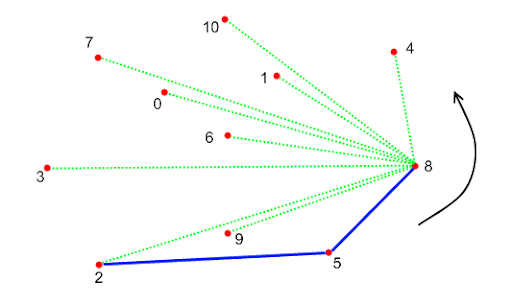
\includegraphics[width=0.8\textwidth]{images/jarvis.png}\\[5mm]
    \caption{Алгоритм Джарвиса}
    \label{Алгоритм Джарвиса}
\end{figure}

Пусть дан массив точек {P} и массив точек {H}. {H} - это массив, куда мы будем записывать точки, состовляющую выпуклую оболочку.\\[2mm]

1. Необходимо найти точку, которая гарантировано будет входить в выпуклую оболочку; очевидно, что самая левая нижняя точка подходит под это условие. Находим точку с минимальной координатой {x} и {y}, и делаем ее текущей {H[0]}.

2. Перебираем все оставшиеся точки двойным циклом по {i} и {j}. В массив H записываем самую правую точку относительно вектора {H[i]P[j]}. Для этого находим векторное произведение, и если оно меньше 0, следовательно точка {P[j]} находится правее точки {P[i]} относительно {H[i]}.

3. Алгоритм завершается тогда, когда в {H} будет записана стартовая вершина и следовательно линия замкнется.

\subsection{Алгоритм проверки правильности решения}

Алгоритм проверки правильности решения определяет пхождение каждой точки в выпуклую оболочку.

Пусть у нас есть множество {P} - множество всех точек, и множество {H} - множество точек, образующих выпуклую оболочку.\\[2mm]

1. Поочереди перебираем каждую точку. Если выбранная точка является точкой, входящая в {H}, то пропускаем и идем дальше.

2. Если точка лежит на границе оболочки, то переходим на следующую итерацию.

2. Строим луч, который берет начало в выбранной точке, идет параллельно оси {X} и направлен от оси {Y} (то есть вправо).

3. Если луч пересекает границу оболочки нечетное количество раз, то точка внутри, иначе - вне оболочки.

\newpage
\section{Описание схемы распараллеливания}

Ниже представлена схема распараллеливания.

\begin{figure}[h!]
    \centering
    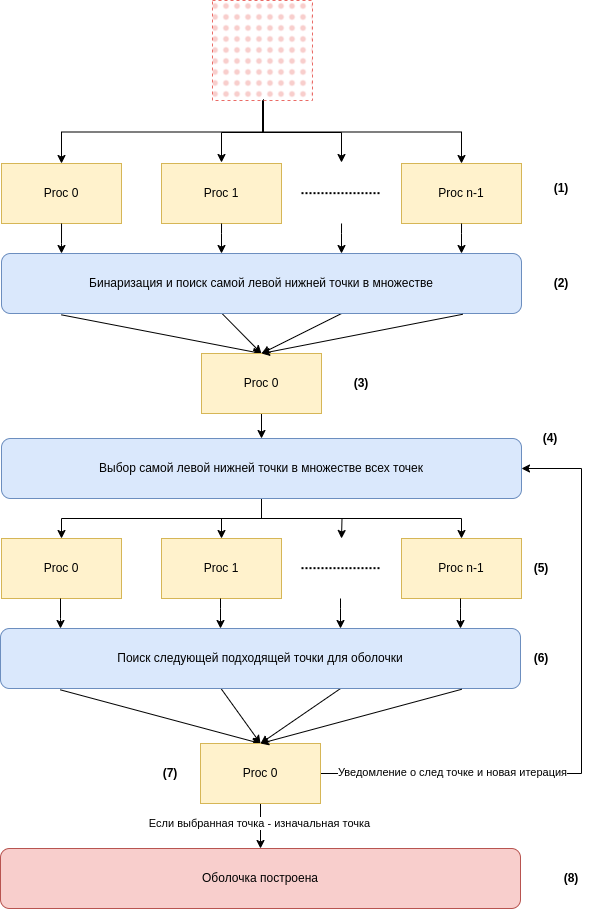
\includegraphics[width=0.8\textwidth]{images/image.png}\\[5mm]
    \caption{Описание схемы распараллеливания}
    \label{Описание схемы распараллеливания}
\end{figure}

\newpage
Описание каждого шага:\\[2mm]

1. Исходное изображение делится между процессами при помощи \texttt{scatterv}. Остаток от деления достается нулевому процессу.

2. Каждый процесс получил свою часть изображения. В этой части каждыый процесс бинаризая изображение, тем самым получая множество $P_i$, где {i} - номер процесса. После каждый процесс в своем множестве находит самю нижнюю левую точку.

3. Все найденные точки собираются на нулевом процессе, используя \texttt{gather}. Нулевой процесс, назовем его \textbf{root}, собрал {n} точек, где {n} - кол-во процессов.

4. root процесс выбирает самую левую нижнюю точку, среди всего множества {P}. После рассылает остальным выбранную точку, при помощи \texttt{broadcast}.

5. Каждый процесс знает начальную точку. В пределах своего множества $P_i$ ищет следующую подходящую точку ддля выпуклой оболочки, используя алгоритм Джарвиса.

6. Все выбранные точки собираются на root процессе через \texttt{gather}, и он выбирает среди них следующую в выпуклую оболочку.

7. Если новая точка это есть начальная точка, то заканчиваем поиск выпуклой оболочки. Иначе - рассылаем с помощью \texttt{broadcast} новую точку всем процессам и идем на новую итерацию алгоритма.

8. Алгоритм закончен, мы построили выпуклую оболочку. Все точки оболочки находятся в первом процессе.


\newpage
\newpage
\section{Результаты экспериментов}
\subsection{Оборудование}


\textbf{Ноутбук}
\begin{itemize}
    \item Процессор AMD Ryzen 7 5700u with radeon graphics × 16
    \begin{itemize}
        \item  Количество ядер - 8
        \item  Количество потоков - 16
        \item  Базовая частота, в гигагерцах - 1.8
    \end{itemize}
    \item RAM - 16ГБ
    \item OS Ubuntu 20.04.6 LTS
\end{itemize}

\begin{center}
    \subsection{Описание эксперимента}
\end{center}

В программе были поставлены счетчики времени, используя \texttt{boost::mpi::timer}. Запуск был осуществлен на 2, 3 и 4 процессах и 5 изображениях разных размеров. Для чистоты эксперимента собиралась статистика 20 запусков и выбиралось среднее значение. Результаты ниже в таблице.\\[2mm]

\begin{center}
\begin{tabular}{ ||c | c | c ||  }
 \hline
 \multicolumn{3}{| c |}{Запуск алгоритма на 2 процессах}\\
 \hline
 Размер изображения ($n \times m$) & Параллельный алгоритм (сек) & Синхронный алгоритм (сек) \\
 \hline
$(9 \times 11)$ & 0.00014204 & 0.00001632 \\
$(100 \times 100)$ & 0.00025598 & 0.00047284 \\
$(200 \times 300)$ & 0.00123358 & 0.00290271 \\
$(400 \times 500)$ & 0.00462814 & 0.00976311 \\
$(500 \times 600)$ & 0.00618927 & 0.01366121 \\
 \hline
\end{tabular}\\[5mm]

\begin{tabular}{ ||c | c | c ||  }
 \hline
 \multicolumn{3}{| c |}{Запуск алгоритма на 3 процессах}\\
 \hline
 Размер изображения ($n \times m$) & Параллельный алгоритм (сек) & Синхронный алгоритм (сек) \\
 \hline
$(9 \times 11)$ & 0.00007188 & 0.00001284 \\
$(100 \times 100)$ & 0.00017434 & 0.00043404 \\
$(200 \times 300)$ & 0.00123358 & 0.00290271 \\
$(400 \times 500)$ & 0.00320425 & 0.00955258 \\
$(500 \times 600)$ & 0.00449706 & 0.01324535 \\
 \hline
\end{tabular}\\[5mm]

\begin{tabular}{ ||c | c | c ||  }
 \hline
 \multicolumn{3}{| c |}{Запуск алгоритма на 4 процессах}\\
 \hline
 Размер изображения ($n \times m$) & Параллельный алгоритм (сек) & Синхронный алгоритм (сек) \\
 \hline
$(9 \times 11)$ & 0.000192573 & 0.00001428 \\
$(100 \times 100)$ & 0.00015547 & 0.00047586 \\
$(200 \times 300)$ & 0.00068672 & 0.00273545 \\
$(400 \times 500)$ & 0.00223551 & 0.00896934 \\
$(500 \times 600)$ & 0.00295943 & 0.01321157 \\
 \hline
\end{tabular}
\end{center}

\newpage
\begin{center}
    \section{Анализ результатов}
\end{center}

Посчитаем средние коеффициенты ускорения по формуле $ p_i = \frac{\sum{\frac{T_{si}}{T_{pi}}}}{5} $, где $T_{si}$ - время синхронного алгритма, а $T_{pi}$ время параллельного алогритма для {i} задачи, где $i = {1, 2, ..., 5}$. \\[2mm]

Получаем следующие результаты:\\[2mm]

\begin{center}
\begin{tabular}{ ||c | c ||  }
 \hline
 \multicolumn{2}{| c |}{Коеффициент ускорения}\\
 \hline
 Количество процессов & Ускорение \\
 \hline
2 & 1.56 \\
3 & 1.82 \\
4 & 2.92 \\
 \hline
\end{tabular}
\end{center}

\textbf{Вывод}: ускорение находится в интервале от 1 до {n}.

\textbf{Проверим ответ на логичность.} Исходная сложность алгоритма - $O(N \cdot H)$, где {N} - общее количество точек, {H} - количество точек в выпуклой оболочке. Т.к. сложность больше, чем {O(N)}, то полученный ответ вполне разумный.

\newpage
\begin{center}
\section{Заключение}
\end{center}

Параллельная версия реализации алгоритма бинаризации изображения и поиска выпуклой оболочки является более ыстрой, чем синхронная реализация. Но стоит иметь в виду, что при малых размерах изображения параллельная версия будет показывать более худшие результаты. Это связано из-за больших накладных расходов для взаимодействия между процессами.

\newpage
\begin{center}
    \section{Список Литературы}
\end{center}

\begin{thebibliography}{8}
\bibitem{algorithmica:1}
Алгоритм Джарвиса (первый сайт). URL: \url{https://ru.algorithmica.org/cs/convex-hulls/jarvis/}

\bibitem{habr:1}
Алгоритм Джарвиса (второй сайт). URL: \url{https://habr.com/ru/articles/144921/}

\bibitem{cgraph:1}
Алгоритм Джарвиса (третий сайт). URL: \url{https://cgraph.ru/node/327}

\bibitem{wikipedia:2}
Выпуклая оболочка. URL: \url{https://ru.wikipedia.org/wiki/%D0%92%D1%8B%D0%BF%D1%83%D0%BA%D0%BB%D0%B0%D1%8F_%D0%BE%D0%B1%D0%BE%D0%BB%D0%BE%D1%87%D0%BA%D0%B0}

\bibitem{boost:2}
Boost MPI. URL: \url{https://www.boost.org/doc/libs/1_61_0/doc/html/mpi/tutorial.html}

\bibitem{gigachat:1}
GigaChat: URL: \url{https://developers.sber.ru/gigachat}

\bibitem{creat:1}
Сайт по созданию схем. URL: \url{https://products.aspose.app/diagram/ru/flowchart}

\bibitem{git:1}
GitHub. URL: \url{https://github.com/Atikin-NT/ppc-2023-mpi}
\end{thebibliography}

\newpage
\begin{center}
    \section{Приложение}
\end{center}

\begin{lstlisting}[language=C++,caption=Создание изображения]
std::vector<std::vector<int>> create_image(int n, int m) {
    std::random_device rd;
    std::uniform_int_distribution<int> unif(0, 255);
    std::vector<std::vector<int>> image(n, std::vector<int> (m));
    int i, j;
    for (i = 0; i < n; i++)
        for (j = 0; j < m; j++)
            image[i][j] = unif(rd);
    image[0][0] = 255;  // minimum one point

    return image;
}
\end{lstlisting}

\bigbreak

\begin{lstlisting}[language=C++,caption=Бинаризация изображения]
std::vector<std::pair<int, int>> get_points_from_image(const std::vector<std::vector<int>> &image, int n) {
    boost::mpi::communicator world;

    int rank = world.rank();
    int delta = n / world.size();


    std::vector<std::pair<int, int>> points;
    for (int i = 0; i < image.size(); i++)
        for (int j = 0; j < image[0].size(); j++)
            if (image[i][j] > 178)
                points.emplace_back(j, rank * delta + i);
    return points;
}
\end{lstlisting}

\newpage
\begin{lstlisting}[language=C++,caption=Параллельная версия Джарвиса]
std::vector<P> JarvisParallel(const std::vector<std::vector<int>> &image, int n) {
    boost::mpi::communicator world;
    int rank = world.rank();
    int commsize = world.size();

    std::vector<P> result;
    std::vector<std::pair<int, int>> selected_points(commsize, std::make_pair(image[0].size(), image[0].size()));
    std::pair<int, int> start_point = std::make_pair(image[0].size(), image[0].size());

    std::vector<std::pair<int, int>> points = get_points_from_image(image, n);
    for (auto p : points)
        if (p.second < start_point.second || (p.second == start_point.second && p.first < start_point.first))
            start_point = p;

    boost::mpi::gather(world, start_point, selected_points.data(), 0);
    if (rank == 0) {
        for (auto p : selected_points)
            if (p.second < start_point.second || (p.second == start_point.second && p.first < start_point.first))
                start_point = p;
    }
    boost::mpi::broadcast(world, start_point, 0);

    if (points.empty())
        points.emplace_back(start_point);

    std::pair<int, int> current = start_point;
    std::pair<int, int> next_point = points[0];

    while (true) {
        for (auto p : points) {
            if (p == current)
                continue;
            int val = crossProduct(current, next_point, p);
            if (val > 0) {
                next_point = p;
            } else if (val == 0) {
                if (distance(current, next_point, p) < 0)
                    next_point = p;
            }
        }

        boost::mpi::gather(world, next_point, selected_points.data(), 0);

        if (rank == 0) {
            for (auto p : selected_points) {
                if (p == current)
                    continue;
                int val = crossProduct(current, next_point, p);
                if (val > 0) {
                    next_point = p;
                } else if (val == 0) {
                    if (distance(current, next_point, p) < 0)
                        next_point = p;
                }
            }
            result.emplace_back(next_point);
        }
        boost::mpi::broadcast(world, next_point, 0);
        current = next_point;

        if (next_point == start_point)
            break;
    }
    return result;
}
\end{lstlisting}

\bigbreak

\begin{lstlisting}[language=C++,caption=Синхронная версия Джарвиса]
std::vector<P> Jarvis(std::vector<std::pair<int, int>> points) {
    std::pair<int, int> start_point = points[0];
    for (auto p : points)
        if (p.second < start_point.second || (p.second == start_point.second && p.first < start_point.first))
            start_point = p;

    std::vector<P> result;
    std::pair<int, int> current = start_point;
    std::pair<int, int> next_point = points[0];
    while (true) {
        for (auto p : points) {
            if (p == current)
                continue;
            int val = crossProduct(current, next_point, p);
            if (val > 0) {
                next_point = p;
            } else if (val == 0) {
                if (distance(current, next_point, p) < 0)
                    next_point = p;
            }
        }

        result.emplace_back(next_point);
        current = next_point;

        if (next_point == start_point)
            break;
    }
    return result;
}
\end{lstlisting}

\newpage
\begin{lstlisting}[language=C++,caption=Проверка вхождения точек в выпуклую оболочку]
bool inside_conv(const std::vector<P> &pol, std::vector<std::pair<int, int>> points) {
    int pol_size = pol.size();
    for (auto point_pair : points) {
        P point(point_pair);
        int j = pol_size - 1;
        bool res = false;
        for (int i = 0; i < pol_size; i++) {
            if (pol[i] == point || pol[j] == point || (pol[i].y == pol[j].y && pol[i].y == point.y) ||
                (pol[i].x == pol[j].x && pol[i].x == point.x)) {
                res = true;
                break;
            }
            if ((pol[i].y < point.y && pol[j].y >= point.y || pol[j].y < point.y && pol[i].y >= point.y) &&
                (pol[i].x + (point.y - pol[i].y) / (pol[j].y - pol[i].y) * (pol[j].x - pol[i].x) == point.x)) {
                res = true;
                break;
            }
            if ((pol[i].y < point.y && pol[j].y >= point.y || pol[j].y < point.y && pol[i].y >= point.y) &&
                (pol[i].x + (point.y - pol[i].y) * (pol[j].x - pol[i].x) / (pol[j].y - pol[i].y) > point.x))
                res = !res;
            j = i;
        }
        if (!res)
            return false;
    }
    return true;
}
\end{lstlisting}

\end{document}
